\documentclass{article}
\usepackage{graphicx}
\usepackage{minted}
\usepackage{parskip}
\usepackage[colorlinks,
            urlcolor=blue]{hyperref}
%\usepackage[margin=1in]{geometry}
\usepackage{amsmath}
\usepackage{amssymb}
\usepackage{fancyvrb}
\usepackage{booktabs}
\usepackage{url}
\usepackage{hyperref}
\usepackage{multirow}
\usepackage{pbox}
\usepackage[margin=1in]{geometry}

\author{Ashwin Srinath}
\title{OpenCL-based tridiagonal solvers for evaluation
    of compact finite differences on parallel architectures}

\begin{document}
\renewcommand{\refname}{References}

\maketitle


\begin{abstract}
    We present methods to evaluate compact finite differences in a
    heterogeneous cluster environment
    on two different architectures: NVIDIA GPUs and Intel multicore CPUs.
    Our methods are compared against the CFDNS implementation,
    which uses a parallelized version of the LU algorithm.
    The implementations are tested on the Clemson University Palmetto supercomputer---each
    node is equipped with 2 NVIDIA Tesla K20 GPUs and a
    2.4 GHz 16 core Intel Xeon Processor.
    The OpenCL framework is used to develop platform-independent code
    so that other parallel architectures can be studied.
    For a problem sized $2048^{3}$,
    our GPU implementation on 64 GPUs provides a
    5x speedup against the CFDNS implementation on the equivalent 512 CPU cores,
    and our CPU implementation provides a 2x speedup against
    the CFDNS implementation on 512 CPU cores.
    The speedup is shown to increase with problem size.
    Compiler optimizations are enabled for all three implementations.
    Our methods achieve speedup by exploiting the parallel architecture in two ways:
    (1) employing cyclic reduction (a parallel algorithm) for each grid line (in the case of GPU), and
    (2) solving multiple grid lines concurrently (both CPU and GPU).
    Our GPU implementation uses a novel strategy
    based on precomputing coefficients,
    to improve the memory access pattern,
    and reduce the number of computations involved.
    The results are of direct interest for implementing compact finite difference
    solvers for other parallel architectures, such as MICs.


\end{abstract}


\section{Introduction}

    The motivation for this work comes from the need to evaluate
    \emph{compact finite differences} arising in large CFD simulations.
    Compact finite different schemes result in
    high order of accuracy for relatively small stencils.
    Numerical methods with small stencil widths are especially benefitial
    in managing communication costs in large-scale cluster computing.
    Compact finite difference schemes lead to
    several banded tridiagonal systems,
    the solution of which is generally the most time-consuming step in the simulation process.
    It is thus desirable to exploit available parallel architectures to speed up
    the solution of the tridiagonal systems.
    The target architectures studied are the NVIDIA Tesla K20 GPU,
    and and a 2.4 GHz Intel Xeon processor with 16 cores.
    Other parallel architectures are of interest---specifically the
    Intel Xeon Phi many-integrated core.

    Several recent efforts have been made to exploit massively parallel architectures
    in the solution of tridiagonal systems.
    \cite{Zhang:2010:FTS:1837853.1693472} discuss the GPU implementation of three algorithms
    and their hybrid variants: Cyclic Reduction, Parallel Cyclic Reduction
    and Recursive Doubling.
    Their approach utilizes the GPUs \emph{shared memory},
    and addresses the concerns of bank conflicts arising in these algorithms.
    A global memory implementation of their solvers
    runs about three times slower, but is able to accomodate larger systems.
    The speedups they report are 12x over a 2.5 GHz quad-core CPU.
    \cite{kim2011scalable} and \cite{davidson2011auto} both propose hybrid
    Parallel Cyclic Reduction and thread-level parallel Thomas algorithm (p-Thomas), and
    methods to determine the switching point for the algorithms.
    The speedups reported are 8.3x and 11x over a 3.33 GHz Intel i7 quad-core
    processor and a 3.4 GHz Intel i5 dual-core respectively.
    In \cite{chang2012scalable},
    the authors implement a heterogenous (GPU+MPI) solver using the
    SPIKE algorithm for GPUs with a diagonal pivoting strategy for stability.
    More recently, \cite{zhao2015efficiently} propose a \emph{chunked} cyclic reduction
    strategy for GPUs.
    In \cite{tutkun2012gpu}, the inverse of the coefficient matrix
    is used to solve tridiagonal systems resulting from high-order compact
    finite difference schemes. The work here is for a single GPU.
    \cite{esfahanian2014efficient} demonstrate
    a method to improve memory accesses for Cyclic Reduction
    using a reordering strategy, and apply it to compressible viscous flow
    simulations.

    In this work,
    we demonstrate the performance of a thread-parallel Thomas algorithm
    on multi-core CPUs.
    For GPUs,
    we propose novel variant of Cyclic Reduction algorithm that
    reduces global memory accesses and decreases memory requirements by
    pre-computing coefficients.

\section{Numerical method}

    We consider the following fourth-order
    compact finite difference scheme for evaluating the first derivative,
    with a 3-point stencil:

    \begin{equation}
        \alpha(f^{\prime}_{i-1} + f^{\prime}_{i+1}) + f^{\prime}_i
        =
        a\frac{f_{i+1} - f_{i-1}}{dx}
    \end{equation}

    For the particular scheme used, $\alpha = 1/4$,
    and $ a = 3/4 $.
    It is easily noted that this leads to a tridiagonal system of equations,
    along with a 3-point stencil to evaluate the RHS.
    Further, the left boundary can be treated using the following implicit equation:

    \begin{equation}
        f^{\prime}_1 + 2f^{\prime}_2 = \frac{-5f_1 + 4f_2 + f_3}{dx}
    \end{equation}

    The right boundary ($f^{\prime}_{n}$) is treated by utilizing
    the negative complex-conjugate of the Fourier image of the stencil
    at $f^{\prime}_1$:

    \begin{equation}
        f^{\prime}_{n} + 2f^{\prime}_{n-1s}
        =
        \frac{5f_{n} - 4f_{n-2} 1 f_{n-2}}{dx}
    \end{equation}

    The tridiagonal system that needs to be solved for the derivatives,
    then has the form:

    \begin{equation} \label{eqn:compact-tridiagonal-system}
     \begin{bmatrix}
         1&2\\
         1/4&1&1/4\\
         &1/4&1&1/4\\
         &&1/4&1&1/4\\
         &&&1/4&1&1/4\\
         &&&&&\ddots\\
         &&&&&&\ddots\\
         &&&&&&&\ddots\\
         &&&&&&&2&1
      \end{bmatrix}
      \begin{bmatrix}
          f^{\prime}_1 \\
          f^{\prime}_2 \\
          f^{\prime}_3 \\
          \vdots \\
          \vdots \\
          \vdots \\
          \vdots \\
          f^{\prime}_{n-1} \\
          f^{\prime}_n
       \end{bmatrix}
     =
     \begin{bmatrix}
         -5f_1 + 4f_2 + f_3\\
         f_{3} - f_{1}\\
         f_{4} - f_{2}\\
         \vdots\\
         \vdots\\
         \vdots\\
         \vdots\\
         f_{n} - f_{n-2}\\
         5f_{n} - 4f_{n-1} - f_{n-2}
      \end{bmatrix}
    \end{equation}

    A solution strategy is therefore concerned with the following:

    \begin{enumerate}
        \item{The evaluation of the right hand side.}
        \item{The solution of the resulting matrix system.}
    \end{enumerate}

\section{Reference approach} \label{sec:ref-approach}
    The current approach, developed for the CFDNS \cite{livescu2009cfdns}
    Direct Numerical Simulation solver,
    uses a parallel tridiagonal solver based on the standard LU algorithm,
    but specialized for the solution of a constant matrix.
    The problem is distributed among several ``processes'' and each
    process uses a single CPU core to perform computations.
    Assuming the coefficients of the LU algorithm are precomputed,
    the following steps are required to solve the tridiagonal system
    (only steps for the left-right sweep are listed, the right-left sweep
    consists of similar steps):

    \begin{enumerate}
    \item Precompute the arrays of coefficients of the LU algorithm---
    this is done once, in the beginning of the simulation process, and its cost
    can be neglected.
    \item Evaluate the RHS of the system.
    \item Compute $\hat{\phi_i}$ and $\hat{\psi_i}$ for each grid point $i$,
    with $\hat{\phi_i}$ and $\hat{\psi_i}$ both functions of the precomputed
    coefficient arrays and the right hand side.
    \item Every process posts the rightmost values of its $\hat{\phi_i}$ and $\hat{\psi_i}$,
        $\widetilde{\phi_k}$ and $\widetilde{\psi_k}$.
    \item Using the array of $\widetilde{\phi_k}$ and $\widetilde{\psi_k}$,
        each process computes $\widetilde{x_k}$, and uses it to compute
        $x_i,k = \phi_i + \psi_i\widetilde{x_k}$.
    \end{enumerate}

    The Message Passing Interface (MPI) is used for handling communication
    between processes.

\section{Parallelization strategies}

    % left, lower, right, upper
    \begin{figure}[h]
    \begin{center}
    \includegraphics[trim={{100pt} {150pt} {100pt} {150pt}}, clip, height=200pt]{img/domain.eps}
    \end{center}
    \caption{Problem domain}
    \label{fig:domain}
    \end{figure}
    %
    \begin{figure}[ht]
    \begin{minipage}[b]{0.40\linewidth}
    \begin{center}
    \includegraphics[trim={{50pt} {50pt} {50pt} {50pt}}, clip, height=200pt]{img/one-block.eps}
    \end{center}
    \caption{A subdomain (assigned to a process)}
    \label{fig:block}
    \end{minipage}
    %
    \hspace{0.5cm}
    \begin{minipage}[b]{0.40\linewidth}
    \begin{center}
    \includegraphics[trim={{50pt} {50pt} {50pt} {50pt}}, clip, height=200pt]{img/one-thread.eps}
    \end{center}
    \caption{Single grid line within a subdomain}
    \label{fig:grid-line}
    \end{minipage}
    \end{figure}
    %
    \begin{figure}[h]
    \begin{center}
    \includegraphics[trim={{100pt} {250pt} {100pt} {150pt}}, clip, height=200pt]{img/block-dimensions.eps}
    \end{center}
    \caption{Dimensions of subdomain}
    \label{fig:block-dimensions}
    \end{figure}

    \pagebreak

    The compact finite differences need to be evaluated
    at each grid point in the problem domain,
    shown in \ref{fig:domain}.
    Each grid point is represented as a cell in this representation.
    The domain has been shown as partitioned into subdomains (Figure \ref{fig:block}).

    While evaluating the derivative in the x-direction (say),
    each subdomain is assigned to a \emph{compute unit}, or a \emph{process}
    which may be a single core, a multi-core processor, or a GPU.
    Each subdomain may be thought of as a collection of ``lines'' of grid points
    ---referred to as \emph{grid lines}---in the x-direction (Figure \ref{fig:grid-line}),
    and the entire domain may be thought of as a collection of such subdomains.

    In the reference approach, each subdomain is assigned to a CPU core.
    Each core operates on a subdomain with dimensions as shown
    in the figure \ref{fig:block-dimensions}.
    The computational pattern followed by each core for the steps listed in Section
    \ref{sec:ref-approach}
    is a triple nested loop over the grid points in the subdomain,
    followed by a communication of the ``faces'' of the subdomain with the other
    cores:

    \begin{listing}
    \begin{minted}{fortran}

       do j=1,n2
          do i=1,n1
             x(1,i,j) = bet(1)*x(1,i,j)
             do k = 2, n3
                x(k,i,j) = (x(k,i,j) - a(k)*x(k-1,i,j))*bet(k)
             end do
             p_loc(i,j) = x(n3,i,j)
          end do
       end do

       call MPI_Allgather(p_loc,n1*n2,double_real,p,n1*n2, &
          double_real,comm,error)

    \end{minted}
    \caption{Computational pattern in reference approach}
    \label{listing:triple-loop}
    \end{listing}

    Conceptually, the innermost loop solves the tridiagonal system
    for a single grid line,
    while the outer loops navigate the different grid lines.
    The evalution of such triple loops are found to be the most time-consuming steps
    in the solution process,
    and it is desirable to introduce a second level of parallelism to replace these loops.
    Broadly speaking, there are two forms of parallelism that can be exploited:

    \pagebreak

    \textbf{Thread-level parallelism} \\
        In a multi-threaded environment,
        rather than having a single thread perform the local part
        of the computations for each line,
        it is beneficial to have several threads ``sweep'' through the subdomain,
        each performing the computations for a different tridiagonal system.
        This is a sort of \emph{thread parallel} operation (Figure \ref{fig:thread-parallel}).
        Algorithms that are inherently sequential,
        such as the Thomas algorithm lend themselves easily to thread-level parallelism
        With reference to the triple-loop in Listing 1,
        algorithms employing thread-level parallelism reduce the
        size of the outer two loops.

        \begin{figure}[h]
        \begin{center}
        \includegraphics[trim={{100pt} {250pt} {100pt} {150pt}}, clip, height=200pt]{img/thread-parallel.eps}
        \end{center}
        \caption{Thread-level parallelism}
        \label{fig:thread-parallel}
        \end{figure}

    \textbf{Data parallelism} \\
        Algorithms like Cyclic Reduction and Parallel Cyclic Reduction
        use parallel processors to perform
        perform the same operation at different points in the tridiagonal system.
        They are said to exhibit \emph{data parallelism} (Figure \ref{fig:data-parallel}).
        Although these algorithms perform a larger number of computations
        per step compared to the Thomas algorithm,
        they can take far fewer steps to run,
        depending on the number of available parallel processors.
        With reference to the triple-loop in Listing 1,
        algorithms employing data parallelism reduce the size of the innermost loop.

        \begin{figure}[h]
        \begin{center}
        \includegraphics[trim={{100pt} {200pt} {100pt} {150pt}}, clip, height=200pt]{img/data-parallel.eps}
        \end{center}
        \caption{Data parallelism}
        \label{fig:data-parallel}
        \end{figure}

    In this work, we evaluate the performance of a variant of cyclic reduction
    on the GPU that is both data-parallel and thread-parallel,
    and a thread-parallel implementation of the Thomas Algorithm on
    multi-core CPUs.

    Both implementations are compared against the reference implementation
    described in Section \ref{sec:ref-approach}.
    The thread-parallel implementation of Thomas Algorithm is
    straightforward.
    However, implementation of cyclic reduction on GPUs involves several issues,
    and our algorithm is described in detail in Section \ref{sec:gpu-algorithm}.
    %
    % \subsection{Evaluation of the RHS}
    %
    %     The RHS is evaluated by a 3 point stencil computation of
    %     the following form:
    %
    %     \begin{equation*}
    %         r_i = \frac{3}{4dx} (f_{i+1} - f_{i-1})
    %     \end{equation*}
    %
    %     This pointwise update can be performed easily in parallel
    %     for the internal points (points not close to the boundary of the process).
    %     Near the boundaries, the process will require information from its
    %     neighbours.
    %
    %     Thus, each process will require information from its
    %     neighbouring processes every time the derivative needs to be evaluated.
    %
    %     \begin{figure}[h]
    %     \begin{center}
    %     \includegraphics[trim={{100pt} {250pt} {100pt} {200pt}}, clip, height=200pt]{img/da-domain.eps}
    %     \end{center}
    %     \caption{Distribution of a 2-D domain among processes}
    %     \label{fig:da-domain}
    %     \end{figure}
    %
    %     \begin{figure}[h]
    %     \begin{center}
    %     \includegraphics[trim={{100pt} {250pt} {100pt} {200pt}}, clip, height=200pt]{img/da-local-portion.eps}
    %     \end{center}
    %     \caption{Elements required by a process to evaluate RHS}
    %     \label{fig:da-local-portion}
    %     \end{figure}
    %
    %     Thus, the RHS is evaluated in two steps:
    %
    %     \begin{enumerate}
    %         \item Exchange boundary information with neighbouring processes
    %         \item Evaluate the RHS at each grid point (in parallel)
    %     \end{enumerate}
    %
    %     The GPU is specialized for performing such a large number of independent
    %     computations as required in step 2.
    %     The RHS at each grid point is computing by a single work item
    %     (GPU thread).
    %     Therefore the number of work items scheduled is
    %     equal to the number of points in the local domain.
    %
    %     Another popular strategy is to take advantage of
    %     shared memory, by launching 2-dimensional blocks of work-items,
    %     loading each into shared memory, and streaming the third dimension
    %     in registers.
    %     This approach is discussed in [ref], and is much more effective
    %     for larger stencils---as each thread in a block will access the same
    %     value several times, it is effective to use shared memory as explicitly
    %     controlled cache.

\section{Description of the GPU algorithm} \label{sec:gpu-algorithm}

    \subsection{Cluster-level parallelization strategy}

    The size of the problems solved using the high-order compact finite
    difference schemes discussed is usually much larger than can be accomodated
    on a single compute node.
    The problem domain is thus divided into ``subdomains'' and distributed among
    several processes.
    First, we discuss this cluster level parallelism.
    This strategy is common to both our CPU and GPU solvers,
    and was first proposed in \cite{mattor1995algorithm}

    Given N equations in N variables of the form:

    \begin{align}
    & A =
     \begin{bmatrix}
         b_1 & c_1 \\
         a_2 & b_2 & c_2 \\
             & a_3 & b_3 & c_3 \\
             &     & a_4 & b_4 & c_4 \\
             &     &     &     &  \ddots & c_{N-1}\\
             &     &     &     &     a_N  & b_N
      \end{bmatrix}&
    \end{align}

    each process $p$ is concerned with the solution of a \emph{subsystem}
    of equations:

    \begin{align}
    &L_p =
    \begin{bmatrix}
        b_1^p & c_1^p \\
        a_2^p & b_2^p & c_2^p \\
              & a_3^p & b_3^p & c_3^p \\
              &       & a_4^p & b_4^p & c_4^p \\
              &       &       &       &  \ddots & c_{M-1}^p\\
              &       &       &       &     a_{M}^p  & b_{M}^p
     \end{bmatrix}&
    \end{align}

    For each subsystem, the following equations are solved:

    \begin{align}
        & L_p\boldsymbol{x}_p^R = \boldsymbol{r_p} &  \label{eqn:local-eqn-1} \\
        & L_p\boldsymbol{x}_p^{UH} = (-a_1^p, 0, 0 \hdots 0)^T &  \label{eqn:local-eqn-2} \\
        & L_p\boldsymbol{x}_p^{LH} = (0, 0, 0, \hdots -c_M^p)^T \label{eqn:local-eqn-3} &
    \end{align}

    The general solution is obtained as a linear combination of the above solutions:

    \begin{equation} \label{eqn:linear-combo}
        \boldsymbol{x}_p = {\xi}_p^{UH} \boldsymbol{x}_p^R + {\xi}_p^{LH} \boldsymbol{x}_p^{LH}
    \end{equation}

    Where the parameters ${\xi}_p^{UH}$ and ${\xi}_p^{LH}$ are obtained
    by solving the following ``reduced'' system:

    \begin{equation} \label{eqn:reduced-system}
     \begin{bmatrix}
         x_{1,M}^{LH}   &   -1                                                          \\
         -1             &   x_{2,1}^{UH} &   x_{2,1}^{LH}                               \\
                        &   x_{2,M}^{LH} &   x_{2,M}^{LH}  &  -1                        \\
         &              &   -1           &   x_{3,M}^{UH}  &  x_{1,M}^{LH}              \\
         &              &   &                x_{3,M}^{UH}  &  x_{1,M}^{LH} &    -1      \\
         &              &   &            &   &             \ddots   \\
         &              &   &            &   &             &        \ddots \\
         &  &   &   &   &   &   & -1 x_{P,1}^{UH}
      \end{bmatrix}
    \begin{bmatrix}
        \xi_1^{LH} \\
        \xi_2^{UH} \\
        \xi_2^{LH} \\
        \xi_3^{UH} \\
        \xi_3^{LH} \\
        \vdots \\
        \vdots \\
        \xi_P^{UH} \\
     \end{bmatrix}
     = -
     \begin{bmatrix}
         x_{1,M}^R \\
         x_{2,1}^R \\
         x_{2,M}^R \\
         x_{3,1}^R \\
         x_{3,M}^R \\
         \vdots \\
         \vdots \\
         x_P^R \\
      \end{bmatrix}
  \end{equation}

    The solution procedure is then:

    \begin{enumerate}
        \item Each process solves the three equations
        \ref{eqn:local-eqn-1}-\ref{eqn:local-eqn-3}.
        \item Each process communicates the parameters required to
        assemble the ``reduced'' system \ref{eqn:reduced-system}.
        \item The reduced system is solved for the coupling coefficients
        $\xi_i^{UH}$ and $\xi_i^{LH}$, which are sent to their respective processes
        (if required)
        \item Each process solves \ref{eqn:linear-combo} for the local part
        of the solution to the global system.
    \end{enumerate}

    In the context of solving tridiagonal systems arising in compact finite differeces,
    we note the following:

    \begin{enumerate}
        \item Each process solves equations \ref{eqn:local-eqn-1}-\ref{eqn:local-eqn-3}
            for \emph{each grid line} in its subdomain.
        \item The left-hand side of these equations is the same
            for each grid line, coming from equation \ref{eqn:compact-tridiagonal-system}).
        \item The right-hand side for equations \ref{eqn:local-eqn-1} and
            \ref{eqn:local-eqn-2} are the same for each grid line.
            Thus, the equations need only be solved for a single grid line.
        \item Only \ref{eqn:local-eqn-3} is evaluated for each grid line
            in the subdomain. This is expected to be the most computationally expensive step.
    \end{enumerate}


    \subsection{GPU architecture}

        \begin{figure}[h]
        \begin{center}
        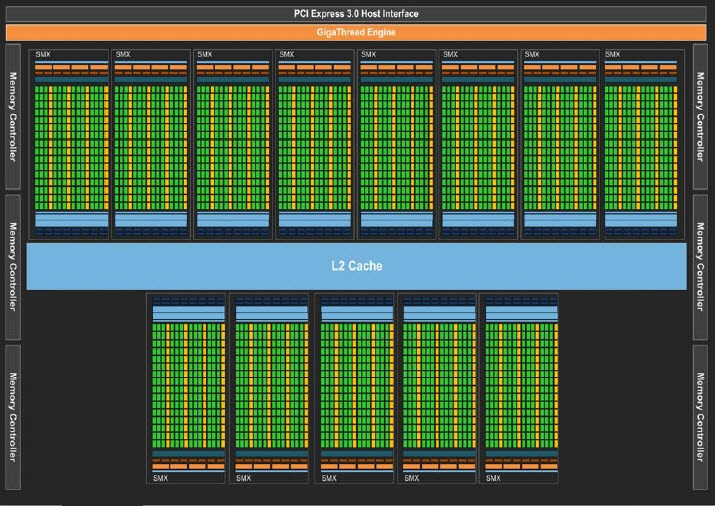
\includegraphics[height=200pt]{img/tesla-block-diagram.jpg}
        \end{center}
        \caption{Block diagram of the K20 GPU}
        \label{fig:k20}
        \end{figure}

        GPUs afford massive parallelism by virtue of several (thousand)
        lightweight compute \emph{threads} or \emph{work-items}.
        The threads on a GPU are scheduled as \emph{blocks},
        which can be 1-D, 2-D, or 3-D.
        Each block is assigned to a \emph{streaming multiprocessor} (SM)
        on the GPU---the Tesla K20 GPU (Figure \ref{fig:k20})
        has 13 streaming multiprocessor---and
        all threads in a block are executed simultaneously by the SM.
        All SMs (and therefore all threads) have access to the GPU's ``global'' memory.
        Access to global memory is efficient when concurrent threads
        access neighbouring memory locations
        (known as \emph{coalesced memory access}).
        All threads in an SM also have access to a common fast, on-chip, \emph{shared memory}.
        Access to shared memory, in general, is much faster than access to global memory,
        but the amount of shared memory per SM is limited, typically a few dozen KB.
        Certain memory access patterns by concurrent threads to shared memory may result in
        serialization of the memory accesses, known as bank conflicts.



    \subsection{Cyclic reduction}

        The classic Cyclic Reduction algorithm consists of two phases:
        forward reduction and backward substitution.
        The forward substitution phase begins with a system of size $N$,
        and by expressing every even-indexed equation $i$ as a linear
        combination of equations $i$, $i-1$ and $i+1$, reduces it to a
        system of size $N/2$.
        The process is repeated until a system of 2 equations in 2 unknowns
        is left.

        For each even-indexed $i$, we define:

        \begin{equation*}
        k_1 = \frac{a_i}{b_{i-1}},
        k_2 = \frac{c_i}{b_{i+1}}
        \end{equation*}

        Then, we update the values of $a$, $b$, $c$ and $d$ as:

        \begin{align} \label{eqn:forward-reduction}
        & a^{\prime}_i = -a_{i-1}k_1 & \\
        & b^{\prime}_i = b_i - c_{i-1}k_1 - a_{i+1}k_2 & \\
        & c^{\prime}_i = -c_{i+1}k_2 & \\
        & d^{\prime}_i = d_i - d_{i-1}k_1  - d_{i+1}k_2 &
        \end{align}

        The two equations are solved, yielding $x_N$ and $x_{N/2}$.
        In the backward substitution phase, every odd-indexed unknown $x_i$
        is solved for by substituting the known values of $x_{i-1}$ and $x_{i+1}$:

        \begin{align} \label{eqn:back-substitution}
        x_i = \frac{d^{\prime}_i - a^{\prime}_ix_{i-1} - c^{\prime}_ix_{i+1}}{b^{\prime}_i}
        \end{align}

        At each step, for the last index $i$, the forward reduction step is
        instead:
        \begin{align} \label{eqn:forward-reduction-right}
            & a^{\prime}_i = -a_{i-1}k_1 & \\
            & b^{\prime}_i = b_i - c_{i-1}k_1 & \\
            & d^{\prime}_i = d_i - d_{i-1}k_1 &
        \end{align}

        And the backward substitution step for $i=1$ is instead:
        \begin{align} \label{eqn:back-substitution-right}
        x_i = \frac{d^{\prime}_i - c^{\prime}_ix_{i+1}}{b^{\prime}_i}
        \end{align}

        \begin{figure}[h]
        \begin{center}
        \includegraphics[trim={{50pt} {300pt} {100pt} {50pt}}, clip, height=200pt]{img/forward-reduction.eps}
        \end{center}
        \caption{Cyclic reduction: memory access pattern for forward reduction}
        \label{fig:forward-reduction}
        \end{figure}

        The cyclic reduction algorithm is well suited to the massively
        parallel architecture of the GPU.
        In the most straightforward implementation,
        we may launch a number of threads equal to
        half the number of equations,
        and assign each thread the task of
        solving the equations \ref{eqn:forward-reduction} for each even-indexed
        $i$.
        We can then perform the successive steps of forward reduction
        by halving the number of threads at each step.
        The backward substitution phase is completed in a similar way,
        with the number of threads doubling at each step.

        This naive approach leads to the following issues:

        \begin{enumerate}
            \item Most of the threads are inactive,
            except at the very beginning of forward reduction
            and the very end of backward substitution.

            \item The later steps of forward reduction and the first few
            steps of backward substitution involve memory accesses with
            large strides (see Figure \ref{fig:forward-reduction})
            If the threads are accessing global memory,
            this can lead to poor performance.
        \end{enumerate}

        The first issue is fairly straightforward to tackle.
        The OpenCL API allows \emph{scheduling} of a large number of
        threads---far more than the number of threads actually available
        on the computing device.
        Rather than scheduling threads for a single system (grid line),
        we may schedule threads to perform
        forward reduction steps for every grid line.
        This ensures that threads that would otherwise be inactive
        now perform computations for other grid lines.

        To avoid non-coalesced accesses to global memory,
        we can instead have threads working with the fast, on-chip,
        \emph{shared memory}. In this case, the threads in each
        \emph{block} read data from global memory on to the block's
        shared memory.
        The threads then perform cyclic reduction on shared memory
        and write the data back to global memory.
        Conceptually, this approach has the advantage of avoiding
        non-coalesced global memory accesses, and facilitates data reuse.
        However, as described in \cite{Zhang:2010:FTS:1837853.1693472}, the method
        suffers from so-called \emph{bank conflicts} in which,
        for certain memory access patters,
        data access by concurrent threads from shared memory may be serialized.
        This can seriously affect performance.
        Several approaches for avoiding bank conflicts have been proposed,
        this is at the cost of additional code complexity.
        Besides, an approach using shared memory suffers from the penalty
        of \emph{synchronization} between blocks and inactive threads.

    \subsection{Precomputing scheme}

        \begin{figure}[h]
        \begin{center}
        \includegraphics[trim={{50pt} {300pt} {100pt} {50pt}}, clip, height=200pt]{img/forward-reduction-coefficients.eps}
        \end{center}
        \caption{Forward reduction: indices with identical coefficients are shown in color}
        \label{fig:forward-reduction-coefficients}
        \end{figure}

        We introduce a variant of cyclic reduction,
        specialized for constant tridiagonal systems, that:

        \begin{enumerate}
        \item Reduces the number of accesses to global memory
        \item Reduces the memory requirement
        \item Reduces the number of computations in the forward reduction step
        \end{enumerate}

        We recall the form of the tridiagonal matrix:

        \[
        \begin{bmatrix}
            1&2\\
            1/4&1&1/4\\
            &1/4&1&1/4\\
            &&1/4&1&1/4\\
            &&&1/4&1&1/4\\
            &&&&&\ddots\\
            &&&&&&\ddots\\
            &&&&&&&\ddots\\
            &&&&&&&2&1
         \end{bmatrix}
         \]

        The matrix is the same for each grid line in the subdomain.
        Thus,
        the first three equations in \ref{eqn:forward-reduction}
        are the same for every grid line.
        For each forward reduction step,
        the parameters $a^{\prime}_i$, $b^{\prime}_i$ and $c^{\prime}_i$
        can be pre-computed.
        For a general tridiagonal system, this would require storage for
        $N/2 + N/4 + ... = 2N-2$ coefficients.
        However, it is readily apparent that,
        with the exception of the boundaries (near the first and last equations),
        the coefficients $k_1$, $k_2$,
        $a_i$, $b_i$ and $c_i$ are the same for each $i$.

        The size of the precomputed coefficient arrays is then $log_2(N)-1$
        (with an additional element for $a_N$ and $b_N$ as described below).
        For event modestly sized $N$ such as 512, this represents large savings
        in the memory requirements for the coefficient arrays.

        More importantly, at each forward reduction step,
        the number of non-coalesced memory accesses is greatly reduced.
        With the above precomputed coefficients,
        the forward reduction step now involves solving only a single equation
        for $d_i$ at each $i$.

        \begin{align} \label{eqn:forward-reduction-right}
            & a^{\prime}_i = -a_{i-1}k_1 & \\
            & b^{\prime}_i = b_i - c_{i-1}k_1 & \\
            & d^{\prime}_i = d_i - d_{i-1}k_1 &
        \end{align}

        The backward substitution step benefits from improved access to
        global memory.

        \subsubsection*{Boundary conditions}

        The tridiagonal systems for all grid lines are the same for all subdomains,
        except near the boundaries.
        From \ref{eqn:forward-reduction}, it is clear that
        to handle the boundaries, three additional sets of coefficients
        need to be stored:

        \begin{enumerate}
         \item The values for $b_1$ at each step
         \item The values for $k_1$ evaluated at $i=1$ for each step
         \item The values for $k_1$ evaluated at $i=n$ for each step,
            where $n$ is the last index of the reduction step.
        \end{enumerate}

        The values of $a_N$ and $b_N$ are required only for the
        final step (2-by-2 solve) of forward reduction.
        These two scalar values may be stored separately.

\section{Performance comparison}

    The reference implementation is compared against our implementations
    of the following algorithms:

    \begin{enumerate}
        \item Cyclic reduction with precomputed coefficients (described above)
            for GPUs
        \item p-Thomas or thread-parallel Thomas algorithm
            for multi-core CPUs
    \end{enumerate}

    In most of the literature, GPU performance is measured
    by comparing the performance of the GPU with
    a single CPU core, or with 2-4 CPU cores.
    We consider a ``node-for-node'' comparison.
    Each node on the Palmetto cluster has 16 CPU cores and 2 GPUs,
    so we maintain a 1:8 ratio of GPUs to CPU cores in our performance evaluation.
    \texttt{O2} level compiler optimizations are applied for the reference implementation,
    the default OpenCL optimizations are applied for our implementations.
    We assume that data loaded on to the GPU is used in other computations
    (evaluation of the RHS, computation of the derivative in other directions),
    and that the computations take long enough that
    the cost of CPU-GPU transfers may be ignored.

    \begin{figure}[h!]
    \begin{center}
    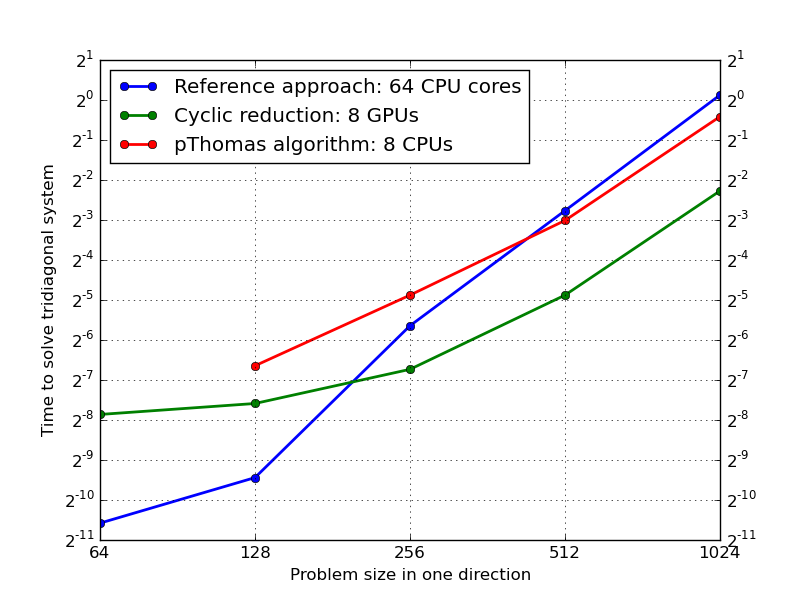
\includegraphics[height=200pt]{results/graphs/4-nodes.png}
    \end{center}
    \caption{Performance of solvers on 4 compute nodes (64 CPU cores, 8 GPUs))}
    \label{fig:4-nodes}
    \end{figure}

    \begin{figure}[h!]
    \begin{center}
    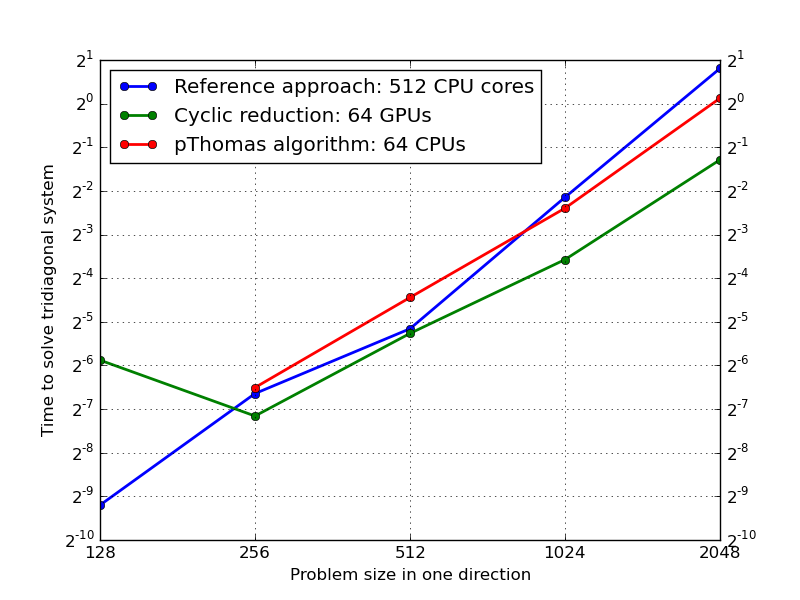
\includegraphics[height=200pt]{results/graphs/32-nodes.png}
    \end{center}
    \caption{Performance of solvers on 32 compute nodes (512 CPU cores, 64 GPUs))}
    \label{fig:32-nodes}
    \end{figure}

    From Figures \ref{fig:4-nodes} and \ref{fig:32-nodes},
    it is clear that the OpenCL implementations run faster than the reference
    implementation for larger problem sizes.
    We also note an increase in the speedup with the problem size.
    For smaller problem sizes,
    the data---specifically for the communication phases of the algorithms---was
    noted to be somewhat noisy.

\section{Performance improvement and future work}

    There is much scope for even better parallel performance and future study.
    Initial profiling results suggest that most of the time is spent solving
    the primary tridiagonal systems,
    but a significant portion of time is spent in assembling and solving
    the secondary ``reduced'' system of equations.
    Our implementations need to be carefully profiled
    to understand where further opimization efforts are required.
    Secondly, finite differences in the other directions can be implemented similarly
    in a straightforward way,
    but it is possible to use a \emph{one-shot}
    strategy, as shown in \cite{esfahanian2014efficient}
    to evaulate all three derivatives concurrently.
    We would also like to develop and evaluate the performance
    a thread-parallel version of the current CFDNS solver,
    which will solve multiple grid lines in a single sweep.
    Finally, we propose to evaluate the performance of our solvers
    on the Intel Many Integrated Core architecture, where we expect to see
    similar results.

    \bibliography{references}
    \bibliographystyle{abbrv}

\end{document}
